% !TEX root = thesis.tex

\chapter{Discussions}
\label{sec:disc}
%\cite{Chatrchyan:2014gia} Measurement of the ratio of inclusive jet cross sections R=0.5 vs R=0.7
%\Dasgupta:2007wa} R dependence of energy 

\section{Comparing dihadron and jet \texorpdfstring{$\jt{}$}{jT} results}
The jet fragmentation transverse momentum $\jt{}$ has been studied previously at ALICE using dihadron correlations~\cite{ALICEjt}. The study took the leading hadron in each event and calculated $\jt{}$ for any near-side tracks with respect to the leading hadron. Thus there is no kinematical limit to $\jt{}$ from the jet cone. In the analysis the background shape is estimated using pairs with large $\Delta \eta$. The normalisation of the background is done when fitting the $\jt{}$ distribution. The inclusive distribution is fitted with a three component function, where one of the components is the background contribution. After subtracting the background, what remains is the signal distribution characterised by the two components. The resulting signal distribution from the analysis is shown in Figure~\ref{fig:dihadron}. The analysis was the first to introduce this factorisation of $\jt{}$ into components.

To constrain the effects from kinematical differences between \pt{,trigger} bins the analysis used bins of the fragmentation variable $\xlong$, which is the projection of the associated particle momentum to the trigger particle normalised by the trigger particle momentum

\begin{equation}
\xlong = \frac{\vec p_t \cdot \vec p_a}{\vec p_t^2}.
\end{equation}

\begin{figure}[htb]
\centering
%\begin{subfigure}{0.49\textwidth}
%\includegraphics[width = 0.95\textwidth]{pics/jtdistribution-89702.pdf}
%\end{subfigure}
%\begin{subfigure}{0.49\textwidth}
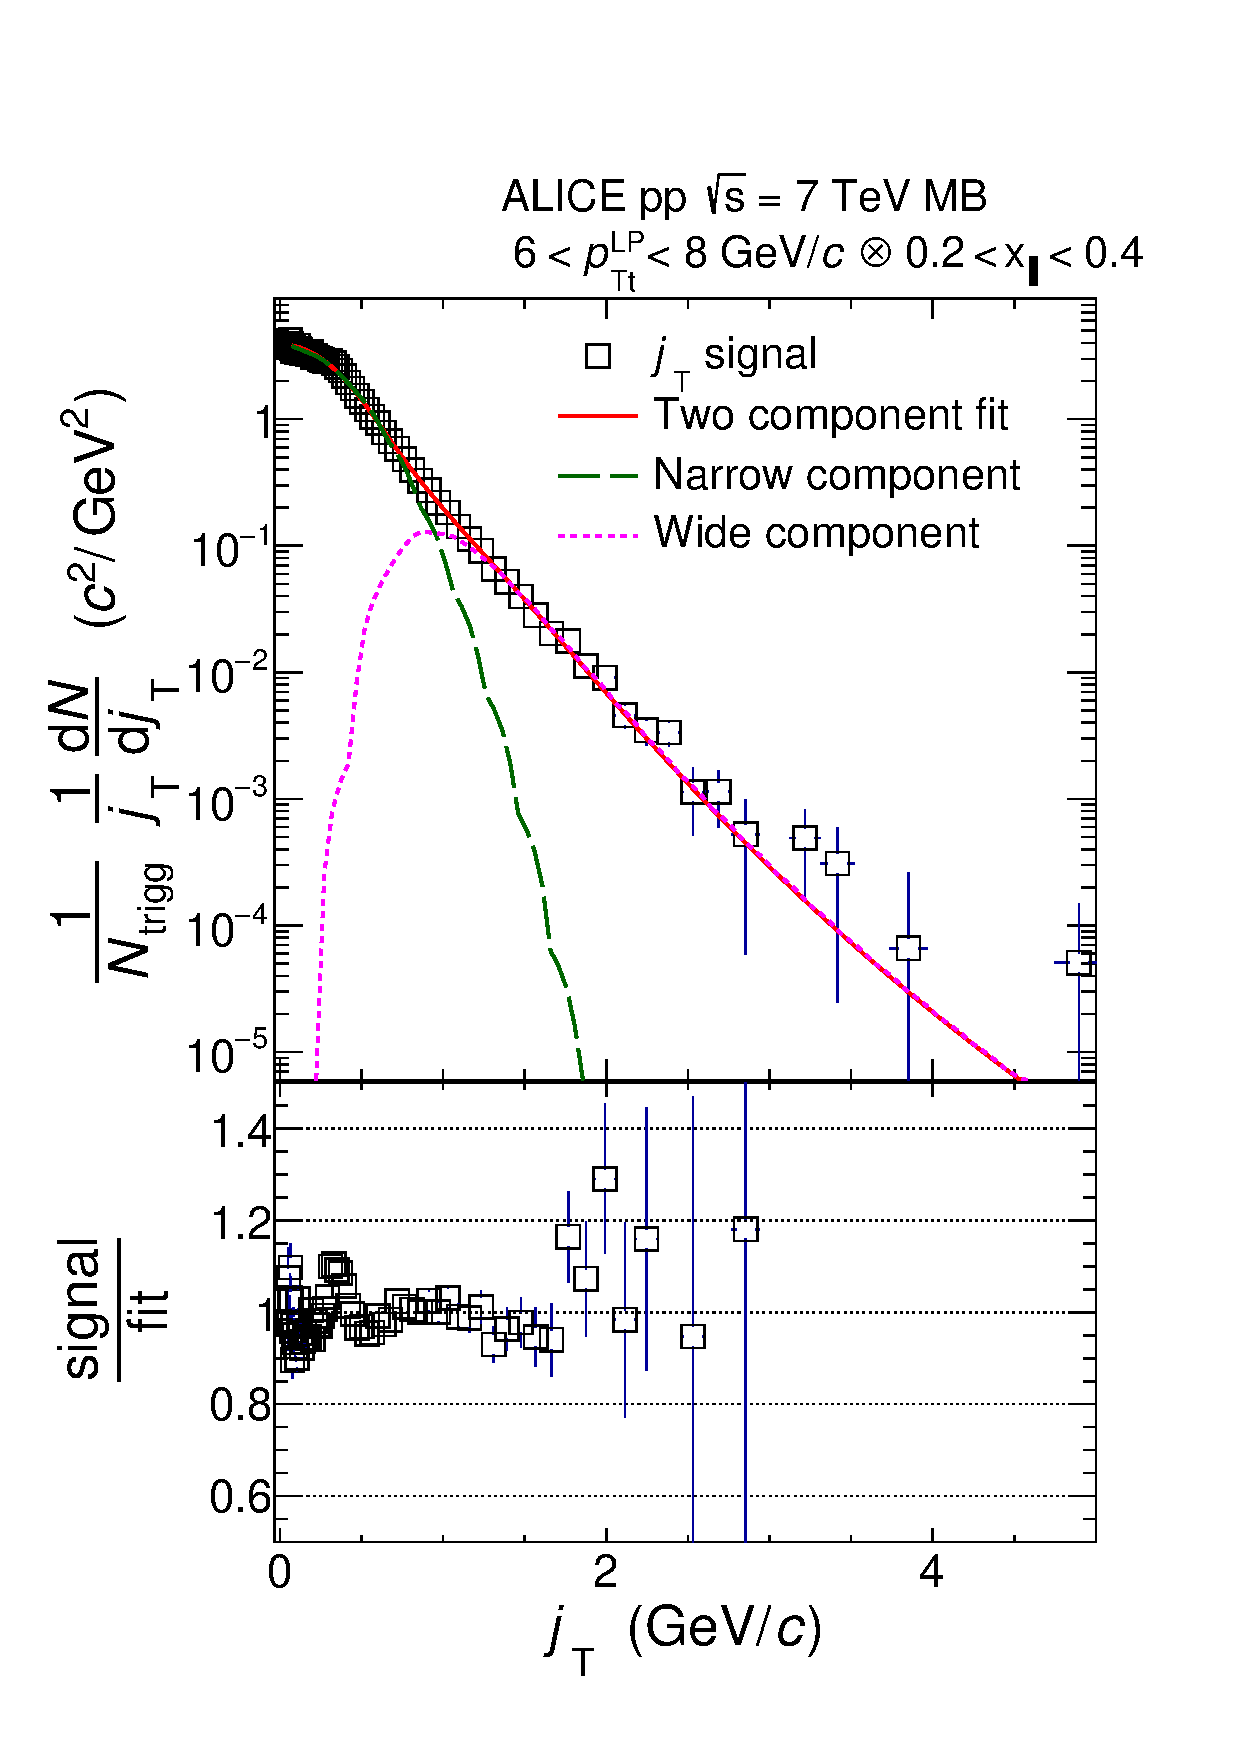
\includegraphics[width = 0.5\textwidth]{pics/jtsignal-89703}
%\end{subfigure}
%\caption[Dihadron $\jt{}$ results]{\emph{Left:} Measured \jt{} distribution including a three-component fit. The three components describe the background (circular symbols), hadronization (long dashed line), and showering (short dashed line). \emph{Right:} The same \jt{} distribution but with background subtracted.}
\caption[Dihadron $\jt{}$ results]{Measured \jt{} signal distribution using dihadron correlations is shown for 6<\pt{t} < 8 and 0.2<\xlong<0.4. The distribution is fitted with the same two component model used in this thesis. Figure from~\cite{ALICEjt}.}

\label{fig:dihadron}
\end{figure}


%\begin{multline}
%\mathrm{Constant\:\times\:background\:+\:Gauss\:+\:Inverse\:Gamma} \\
%B_0 \times\:\mathrm{background} + \frac{B_2}{B_1\sqrt{2\pi}}e^{-\frac{\jt{}^2}{2B_1^2}}+\frac{B_3B_5^{B_4}}{\Gamma\left(B_4\right)}\frac{e^{-\frac{B_5}{\jt{}}}}{\jt{}^{B_4+1}}.
%\end{multline


%At $\jt{} \approx \unit[0.4]{\GeVc}$ there is a small bump in the distribution to fit ratio. This was attributed to cases where the trigger particle decayed after hadronisation. As it is difficult to correct for, this bump is included in the systematic errors of the final results.  


The RMS results from the fitting in both \pp and \pPb collisions are shown in Figure~\ref{fig:dihadronResults}. Qualitatively the results are similar to jet $\jt{}$ results. The RMS value of the wide component has an increasing trend with respect to $\pt{t}/\pt{,jet}$, while the RMS value of the narrow component stays constant. Both components are well described by \pythia~simulations. As seen in the figures there is no difference between minimum bias \pp and \pPb results in the dihadron analysis. 



\begin{figure}[htb]
\centering
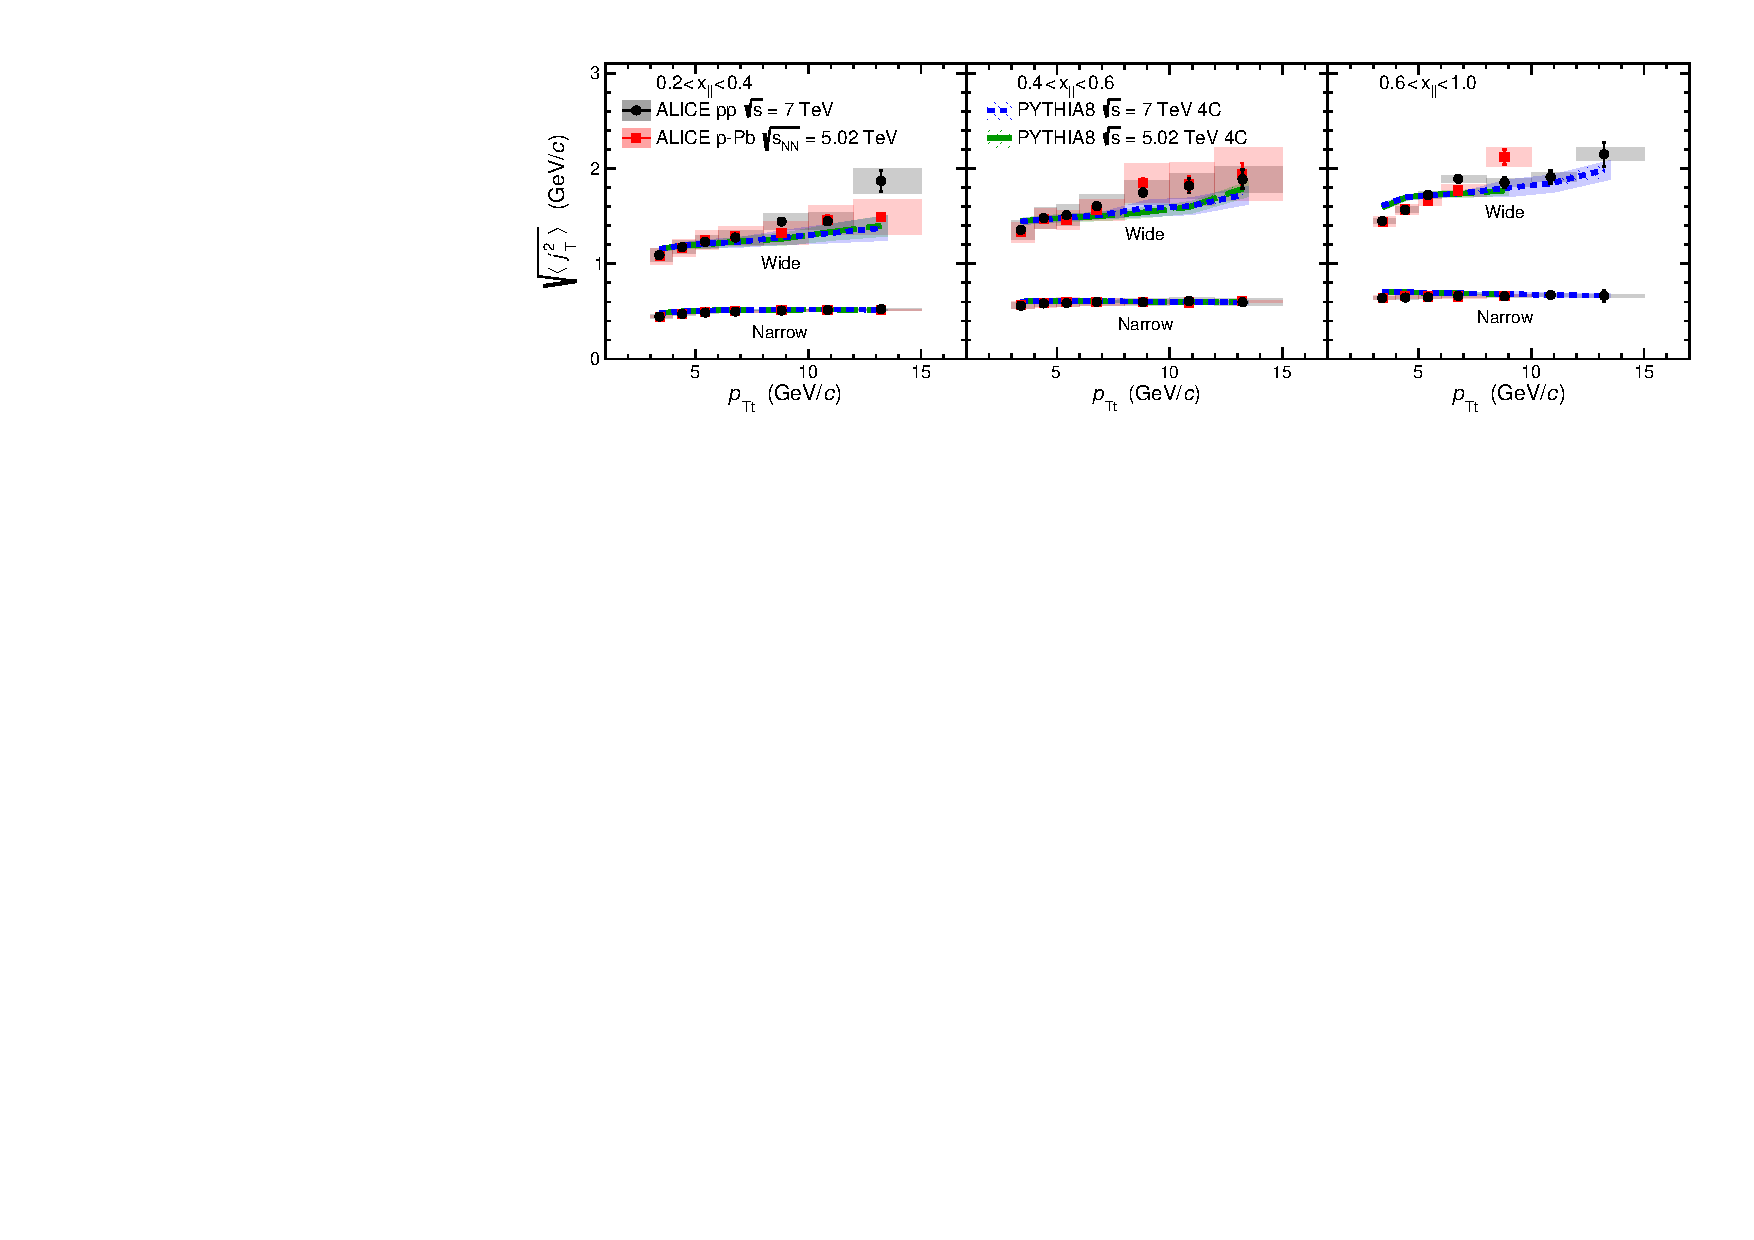
\includegraphics[width=0.99\textwidth]{pics/jt_RMS_finalFormUniformTextSize-89708}
\caption{RMS values of the narrow and wide $\jt{}$ components in the dihadron correlation analysis. Results from \pp collisions at $\sqrt{s} = 7 \tev$ (circular symbols) and from \pPb collisions at \sqrtSnnE{5.02} (square symbols) are compared to \textsc{Pythia}~8 tune 4C simulations at \sqrtSE7 (short dashed line) and at \sqrtSE{5.02} (long dashed line). Different panels correspond to different \xlong bins with 0.2<\xlong<0.4 on the left, 0.4<\xlong<0.6 in the middle, and 0.6<\xlong<1.0 on the right. The statistical errors are represented by bars and the systematic errors by boxes. Figure from~\cite{ALICEjt}.}
%Creative commons license
\label{fig:dihadronResults}
\end{figure}


%\subsection{Comparing dihadron and jet \texorpdfstring{$\jt{}$}{jT} results}
Comparison between RMS values in dihadron \jt{}~\cite{ALICEjt} and jet \jt{} is shown in Figure~\ref{fig:dihadroncomparison}. The dihadron trigger $\pt{}$ bins are converted to jet $\pt{}$ bins and vice versa. Bin-by-bin comparison is still not possible, but general features can be identified. %The most striking difference is that the dihadron analysis gives systematically larger RMS values. This could be caused by several kinematical factors. In jet $\jt{}$ analysis the jet cone limits possible $\jt{}$ values and thus the width and RMS of the $\jt{}$ distributions. The effect of this limitation can be studied by changing the cone size as is described in Section~\ref{sec:Rstudy}. 

%Comparison to $\jt{}$ results from dihadron analysis ~\cite{ALICEjt} is shown in Figure~\ref{fig:DihadronComparison}. 
%Trigger $\pt{}$ bins used in dihadron analysis are converted to jet $\pt{}$ bins using observed average jet $\pt{}$ values in leading track momentum bins. Simlarly jet $\pt{}$ bins are converted to $p_{T,\mathrm{trigger}}$ bins using average leading track $\pt{}$ values in $\pt{,jet}$ bins.

The trends are similar in dihadron and jet $\jt{}$ results. Wide component RMS values tend to increase with increasing $p_{T,\mathrm{trigger}}$/$\pt{,jet}$. For $x_{||}<0.4$ Narrow component RMS increases slightly at low \pt{,trigger} in dihadron analysis. This trend changes between $x_{||}$ bins; In larger $x_{||}$ bins the narrow component RMS is closer to constant as is the case for jet \jt{}.

The most striking difference is that dihadron $\jt{}$ gives wider distributions with larger RMS values. There are several possible causes for this difference. First, in jet analysis the cone size limits width and thus the RMS values. The effect of this limitation can be studied by changing the cone size as is described in Section~\ref{sec:Rstudy}.

Second, the leading track is an imperfect estimate of the jet/original parton. Because the leading track in general is at an angle compared to the jet axis, the resulting $\jt{}$ values are different. In practice the jet axis found by the jet finding algrorithm tends to minimize the average $\jt{}$ of jet constituents. Thus the yield at high $\jt{}$ is limited and the RMS values are smaller. The effect of having the leading hadron as reference instead of the jet axis is discussed in Section~\ref{sec:reference}

Third, the results from the dihadron analysis are done in \pt{,trigger} bins. This favours hard jets, i.e. jets where the leading hadron carries a large momentum fraction and the jet multiplicity is small. In \pt{,jet} bins jets are more likely to be soft, i.e. they have a small leading momentum fraction and high multiplicity jets.



\begin{figure}[htb]
\begin{subfigure}{0.5\textwidth}
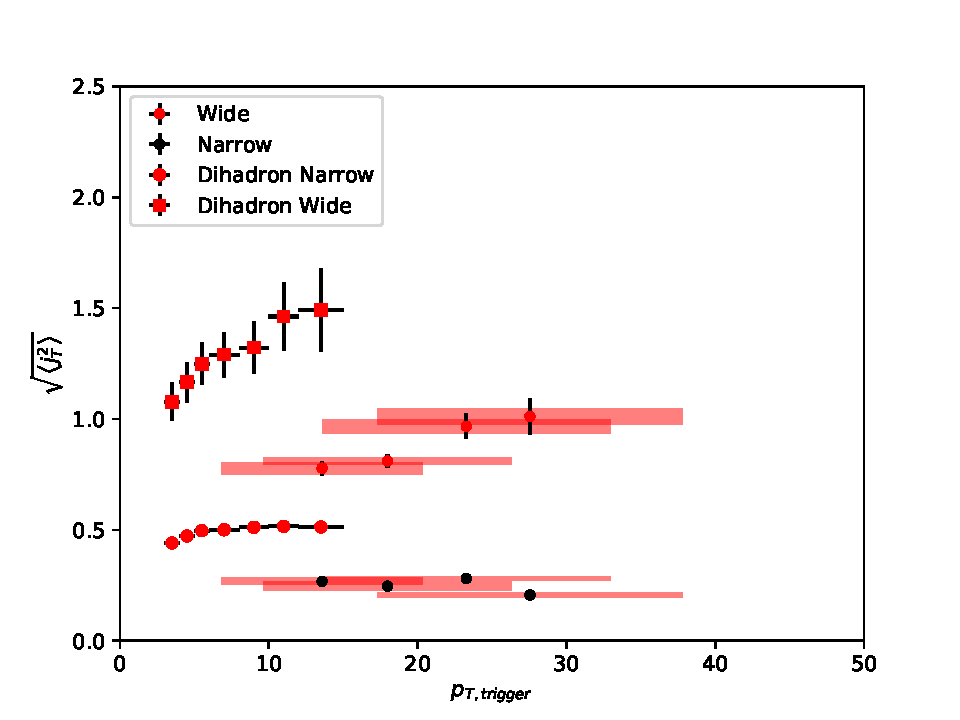
\includegraphics[width=0.99\textwidth]{figures/summary/RMSWithSystematics_DihadronTriggerPt.pdf}
\end{subfigure}
\begin{subfigure}{0.5\textwidth}
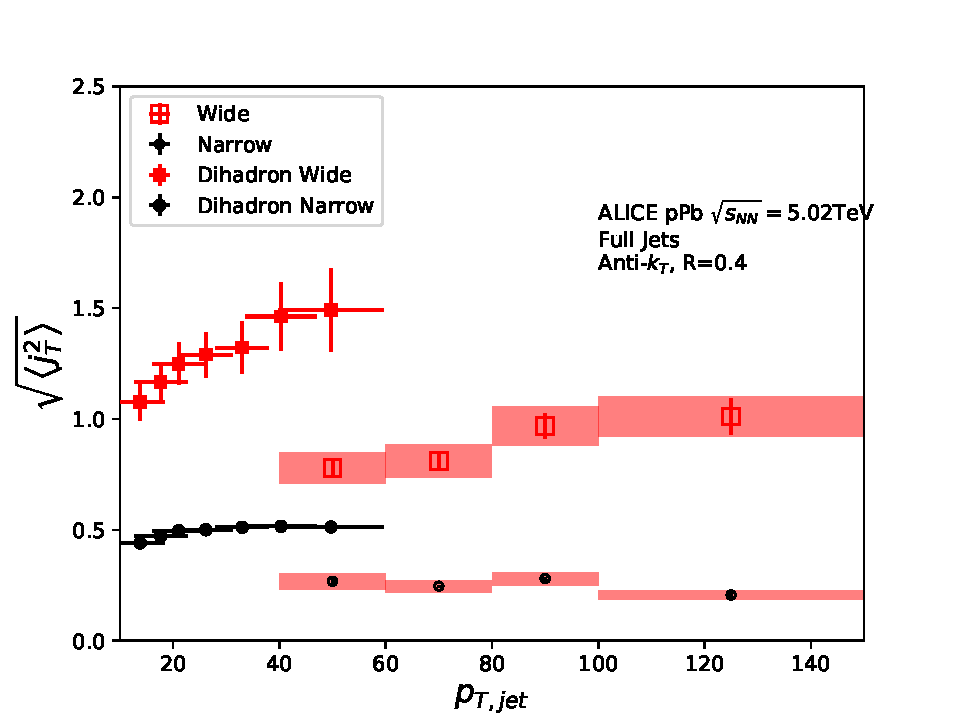
\includegraphics[width=0.99\textwidth]{figures/summary/RMSWithSystematics_DihadronJetPt.pdf}
\end{subfigure}
\caption{Jet $\jt{}$ results are compared to results obtained in the dihadron analysis~\cite{ALICEjt}.. Dihadron trigger $\pt{}$ bins are converted to jet $\pt{}$  bins  using observed mean  $\pt{,jet}$ values in $\pt{,trigger}$ bins. Dihadron results are for $0.2 < x_{||} < 0.4$.}
\label{fig:dihadroncomparison}
\end{figure}

\subsection{Different \texorpdfstring{$R$}{R} parameters}
\label{sec:Rstudy}
The size of the jet cone gives a limit for $\jt{}$. For a track with a fixed momentum $p$ this is a hard limit. This is conveniently seen as $\jt{,max}$ can be given in terms of cone size $R$ and momentum $p$. In the small angle approximation limit

\begin{equation}
\jt{,max} \approx p \cdot R.
\end{equation}

\noindent  Thus for tracks with $\pt{,track} < \pt{0} $, must be $\jt{} < \pt{0} \cdot R$.  This illustrated in Figure~\ref{fig:jtmax}.
\begin{figure}[h!]
\tikzset{
photon/.style={decorate, decoration={snake}, draw=red},
particlearrow/.style={draw=blue, postaction={decorate},
    decoration={markings,mark=at position .5 with {\arrow[draw=black]{>}}}},
antiparticlearrow/.style={draw=blue, postaction={decorate},
    decoration={markings,mark=at position .5 with {\arrow[draw=black]{>}}}},
particle/.style={draw=blue},
antiparticle/.style={draw=blue},
gluon/.style={decorate, draw=orange,
    decoration={coil,amplitude=4pt, segment length=5pt}}
 }
\centering
\begin{tikzpicture}[scale= 3]
\coordinate[] (a);
\coordinate[above right = 1.2cm and 3cm of a,label=right:{\color{black!60}Jet Cone}] (b);
\coordinate[below right = 1.2cm and 3cm of a] (c);
\coordinate[above right = 0.8cm and 2cm  of a] (d);
\coordinate[below right = 1.1cm and 2cm  of a] (h);

\coordinate[right = 2cm of a] (e);
\coordinate[right = 4cm of a] (g);
\coordinate[right = 3cm of a] (f);
\draw[thick, black!60] (a) -- (b);
\draw[thick, black!60] (a) -- (c); 
\draw[thick, blue,->] (a) -- node[label=above:$\vec{p}_\mathrm{track}$] {}  (d);
\draw[thick, blue,->] (a) -- node[label=below:$\vec{p}_\mathrm{track}$] {}  (h);
\draw[thick, black!40, ->] (a) -- (g);
\draw[dashed,blue,->] (e) -- node[label=right:$\jt{max}$] {}  (d);
\draw[thick, black!60, ->] (f) --  node[label=right:$R$] {}  (c);
\end{tikzpicture}
\caption{\jt{} has maximum value defined by the cone size and track momentum $\vec{p}_\mathrm{track}$}
\label{fig:jtmax}
\end{figure}
 

We studied the effect of cone sizes on $\jt{}$ distribution with a \pythia~simulation. Distributions with different cone sizes in different \pt{,jet} bins are shown in Figure~\ref{fig:RcomparisonjT}. The increase of high $\jt{}$ with increasing cone size, $R$, is clearly seen in the individual $\jt{}$ distributions. At low $\jt{}$ there is no change within the errors.

When looking at the RMS values from wide component we see an increase or decrease of about 10\% when going from $R=0.4$ to $R=0.5$ or $R=0.3$, respectively. This is seen in Figure~\ref{fig:RcomparisonRMS}. The message from narrow component RMS values is less clear. At low jet $\pt{}$ the behaviour is similar, but at high $\pt{}$ the order is reversed. 


\begin{figure}[htp]
\centering
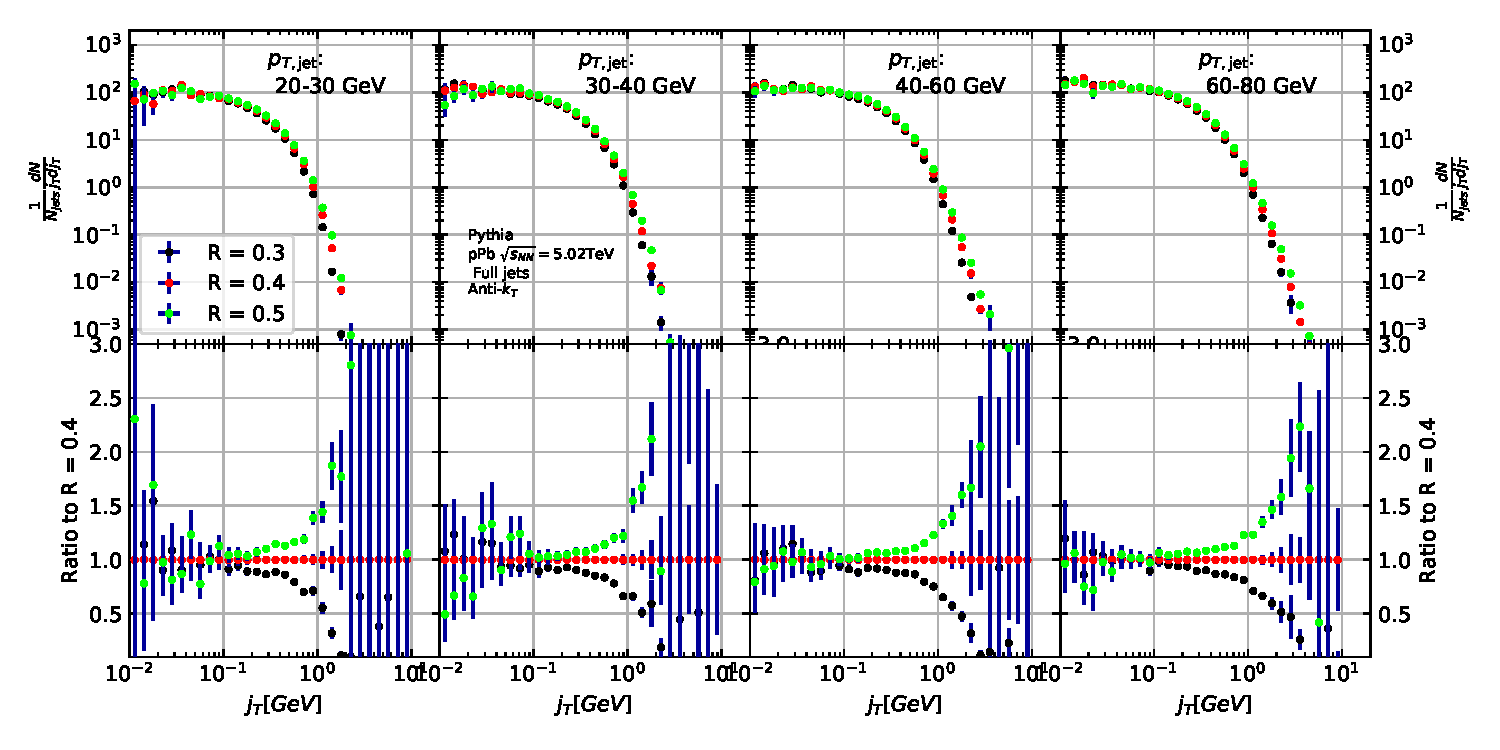
\includegraphics[width=0.97\textwidth]{results/RcomparisonSignal.pdf}
\caption[Pythia $R$ parameters $\jt{}$]{Effect of changing cone size on $\jt{}$ distributions. The change is done both for the $R$  parameter in the anti-\kt{} algorithm, and for the size of the cone where $\jt{}$ is calculated.}
\label{fig:RcomparisonjT}
\end{figure}


\begin{figure}[htp]
\centering
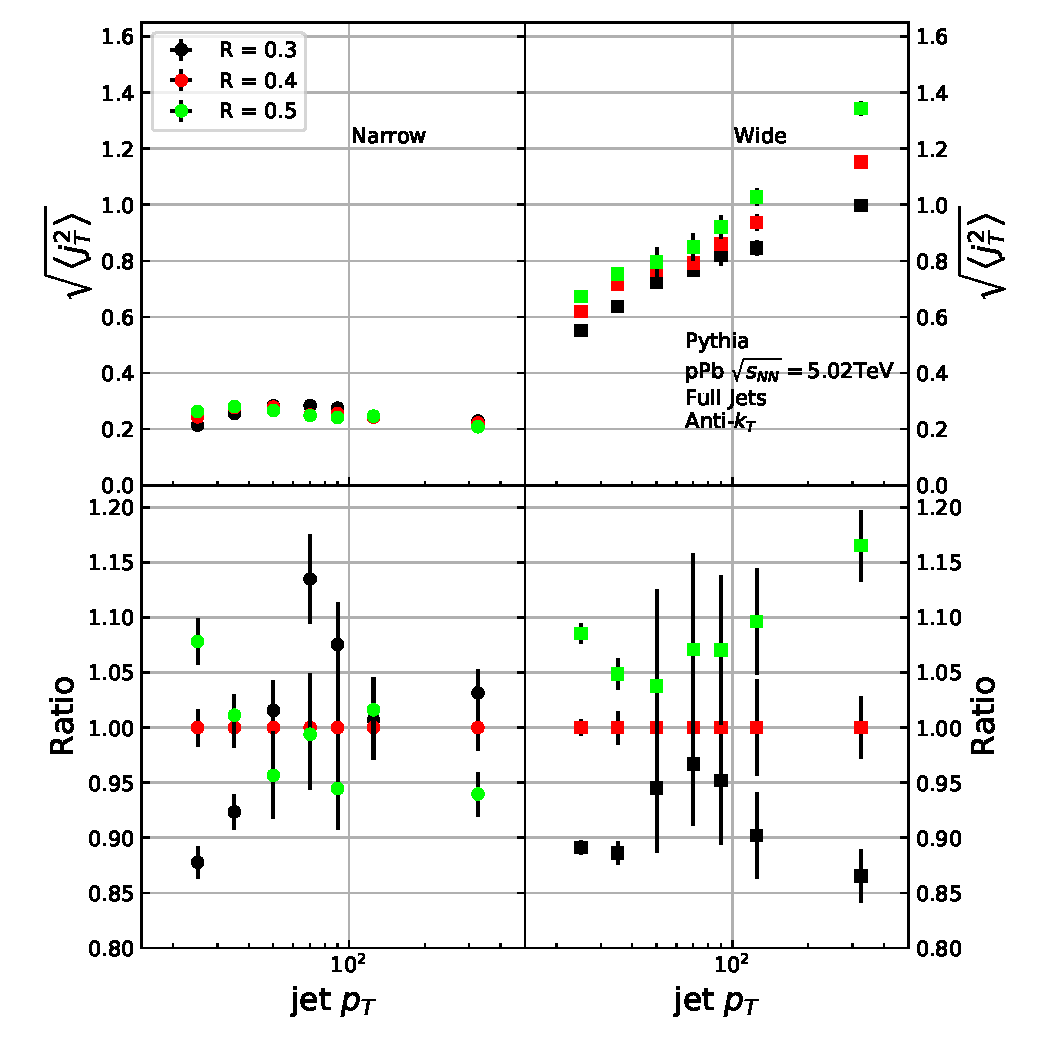
\includegraphics[width=0.6\textwidth]{figures/results/RcomparisonRMS.pdf} \\
\caption[Pythia $R$ parameters RMS]{Effect of changing $R$ parameter in jet finding on narrow and wide component RMS values. Wide component RMS values increase with increasing cone size.}
\label{fig:RcomparisonRMS}
\end{figure}


%Effect of the $R$ parameter choice is studied in \textsc{Pythia}. Having a fixed cone puts hard limits on the possible $\jt{}$ values. Increasing the cone size loosens these limits and allows higher $\jt{}$ values. The results are shown in Figure~\ref{fig:Rcomparison}. Left hand side shows the $\jt{}$ distributions. There is very little change in low $\jt{}$ but at high $\jt{}$ the yield increases. 

%This is also seen in the RMS values shown in the right hand side of Figure~\ref{fig:Rcomparison}, where the change in wide component RMS is about 10\% when going from $R=0.4$ to $R=0.3$ or $R=0.5$. With the narrow component values the situation is less clear. At low jet $\pt{}$ larger $R$ parameter leads to larger RMS values, but at high $\pt{,jet}$ the situation is reversed; increasing the $R$ parameter decreases RMS values.

\subsection{Leading tracks versus jet as reference}
\label{sec:reference}
In comparison to the leading hadron the jet axis from jet reconstruction should provide a better estimate of the original parton. The assumption is that because the leading hadron is an imperfect estimate of the jet axis, low $\jt{}$ tracks should on average be shifted to higher $\jt{}$.

Because the leading track is at an angle compared to the jet axis, the resulting $\jt{}$ values are different. In practice the jet axis found by the jet finding algorithm tends to minimise the average $\jt{}$ of jet constituents, as at least the hardest constituents should be close to the jet axis. Thus the yield at high $\jt{}$ is reduced and the RMS values get smaller. On the other hand, when using the leading hadron as a reference, it is naturally missing from the set of tracks for which \jt{} is calculated. This causes a decrease in the yield at low \jt{}.

We performed a \pythia~study where $\jt{}$ was calculated with respect to the leading track momentum, instead of the jet axis. The results are shown in Figure~\ref{fig:RefComparison}. The resulting $\jt{}$ distributions are significantly wider than $\jt{}$ distributions from using the jet axis as reference. The effect seems to be larger than that seen in comparing different $R$ values. 

\begin{figure}[htp]
\centering
\begin{subfigure}{0.59\textwidth}
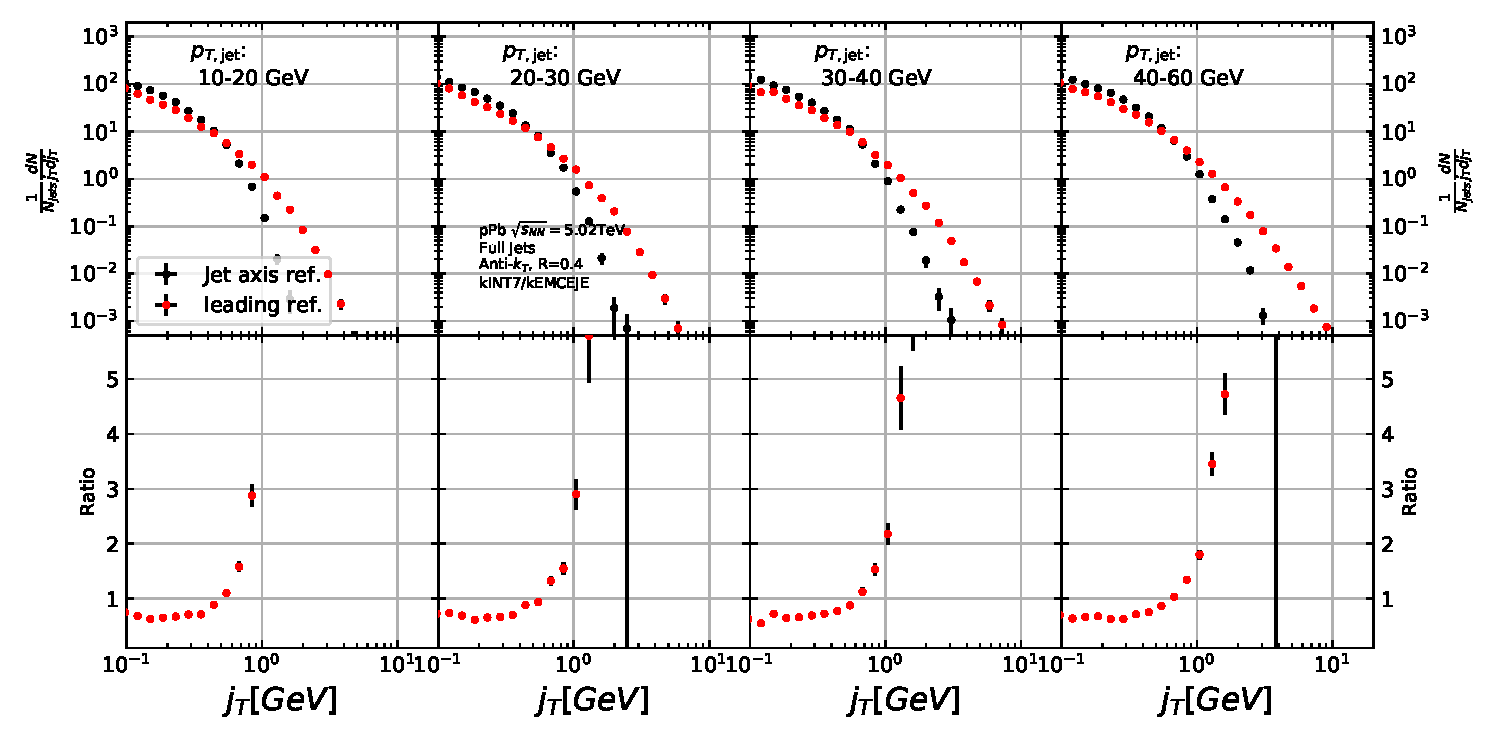
\includegraphics[width=0.99\textwidth]{figures/results/JetVsLeadingRefConst.pdf}
\end{subfigure}
\begin{subfigure}{0.39\textwidth}
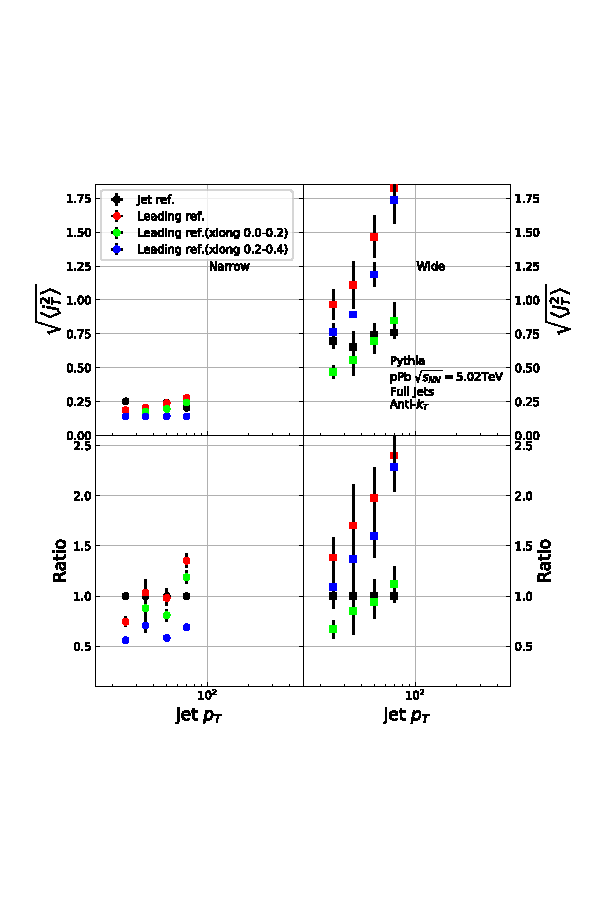
\includegraphics[width=0.99\textwidth]{figures/summary/RMSleadinghadron.pdf}
\end{subfigure}
\caption{Results of calculating $\jt{}$ with respect to the leading hadron, instead of the jet axis in a \pythia~simulation are shown.}
\label{fig:RefComparison}
\end{figure}

A direct comparison between jet and dihadron $\jt{}$ measurements is not possible. But combined with the $R$ dependence of $\rms{\jt{}}$ the difference between $\rms{\jt{}}$ values in jet and dihadron analyses can be quantitively understood. 

\FloatBarrier
\clearpage
\pagebreak
\chapter{Summary}
\label{sec:sum}
In this thesis I have studied the jet fragmentation transverse momentum at $\snn = \unit[5.02]{\tev}$ in \pPb collisions. The analysis was performed using jets reconstructed with the anti-$\kt{}$ algorithm. The resulting $\jt{}$ distributions were fitted with a two component model, which allows us to separate two distinct components. The width of the narrow component was found to depend weakly on jet \pt{}. The narrow component has been associated with the non-perturbative hadronisation process. This is consistent with the assumption that hadronisation is universal, i.e. it doesn't depend on the hard scattering. 

The width of the wide component was found to get larger with increasing $\pt{,jet}$. This is in part explained by the changing kinematical limits when going to higher $\pt{,jet}$ which allows higher $\pt{,track}$. Additionally the larger phase space allows stronger parton splitting.

Both the narrow and wide component RMS values were well described by \pythia~, but Herwig gave larger RMS values for the wide component than data. %\pythia~and Herwig have different algorithms for the showering. 
In the narrow component there was no difference between the models. Both describe the data well. This component was associated with hadronisation. At least in this context the different hadronisation algorithms of \pythia~(string model) and Herwig (cluster model) give similar results.


Similar analysis has been performed with dihadron correlations~\cite{ALICEjt}. Although a direct comparison between the results is not possible, they are qualitatively compatible with each other. The difference is understood to come from the different $\jt{}$ reference, the cone size limitation in jet $\jt{}$ analysis and the kinematical bias that arises from using \pt{,trigger} bins which favours harder jets than using \pt{,jet} bins. The dihadron analysis saw no difference between results in \pp and \pPb datasets and concluded that there were no cold nuclear matter effects. The same is expected to be true for the jet $\jt{}$. This is further supported by the agreement between \pythia~and data as \pythia~results are for \pp collisions. 

To study possible QGP effects in high multiplicity \pPb collisions the analysis was repeated using different multiplicity selections. So far no jet observables have shown conclusive evidence of modification in ~\pPb events. However these are primarily based on measuring yield, which makes them vulnerable to biases when selecting for  multiplicity. Thus these measurements have been only performed in minimum bias events. As $\jt{}$ is based on shape on a per-jet basis, it should not be sensitive to these selection biases. No effect was seen in any of the multiplicity selections. However, with the statistics available, the effect should be quite large ($\gtrapprox 20\%$) to be visible. 

Naturally the next step would be extending the analysis to \PbPb data to gain better understanding of jet modification. Jet analysis in a heavy-ion collision with significant contributions from the underlying event has proved challenging~\cite{Connors:2017ptx}. However, experimental methods have improved in recent years. For the $\jt{}$ analysis presented in this thesis the main challenge would be the background subtraction method. Because of anisotropic flow in heavy-ion collisions the background inside the jet cone and a cone perpendicular to it would be different. It's unclear if the perpendicular cone method can be modified or if a completely new approach is required. 

It has been shown that in \PbPb collisions jets become softer and wider because of medium-induced radiation~\cite{Connors:2017ptx}. On the other hand, the hot medium suppresses gluon jets more than quark jets. This has the opposite effect, narrowing jets, as gluon jets are naturally wider than quark jets~\cite{jetShapeQGP}. How these different effects combine in $\jt{}$ needs to be studied. 